\documentclass[11pt,a4paper]{article}

\usepackage[T1]{fontenc}
\usepackage[utf8]{inputenc}
\usepackage{geometry}
\geometry{margin=2.2cm}

\usepackage{microtype}
\usepackage{hyperref}
\hypersetup{colorlinks=true, linkcolor=black, urlcolor=black}

\usepackage{enumitem}
\setlist[itemize]{leftmargin=*, itemsep=2pt, topsep=2pt}

\usepackage{booktabs}
\usepackage{tabularx}
\usepackage{longtable}
\usepackage{array}

\usepackage{tikz}
\usetikzlibrary{arrows.meta, positioning, shapes.geometric}

\usepackage[most]{tcolorbox}
\tcbset{colback=white, colframe=black!60, sharp corners, boxrule=0.6pt, left=6pt, right=6pt, top=6pt, bottom=6pt}

\newcolumntype{Y}{>{\raggedright\arraybackslash}X}
\newcommand{\DoD}{\textbf{DoD}}

\title{TRACK B --- EVM Engineer (Solidity/Foundry)\\\large Détail exécutable (PDF séparé)}
\author{RBK 2.0}
\date{}

\begin{document}
\maketitle
\tableofcontents
\vspace{6pt}

% =========================================================
\section{Résumé exécutif}
\paragraph{Positionnement.}
Ce track vise un \textbf{EVM Engineer} capable de livrer des smart contracts Solidity \textbf{production-ready} avec une discipline de tests \textbf{professionnelle} (unit, fuzz, invariants), une approche \textbf{security-first}, la maîtrise des standards (ERC) et des patterns industriels (déploiement, verification, upgrades, monitoring).

\paragraph{Promesse mesurable.}
\begin{itemize}
  \item Capacité à produire des contracts avec \textbf{Foundry pipeline complet} (unit $\rightarrow$ fuzz $\rightarrow$ invariants $\rightarrow$ coverage).
  \item Capacité à livrer un projet intégrant \textbf{verification on-chain}, scripts de déploiement reproductibles et \textbf{plan d'upgrade} (UUPS).
  \item Capacité à rédiger un \textbf{mini audit report} et à corriger des findings.
\end{itemize}

\begin{tcolorbox}[title={Non négociables (track B)}]
\begin{itemize}
  \item Tests fuzz et invariants sur les composants critiques.
  \item Threat model + checklist sécurité.
  \item Scripts de déploiement et verification reproductibles.
\end{itemize}
\end{tcolorbox}

% =========================================================
\section{Objectifs mesurables (preuves)}
\begin{table}[h]
\centering
\begin{tabularx}{\textwidth}{l Y Y}
\toprule
\textbf{Domaine} & \textbf{Compétence} & \textbf{Preuve + outil (seuil)} \\
\midrule
Solidity core & Storage/memory/calldata, errors, events, libs &
Repo ``Vault/Escrow'' + tests + doc API \\
Testing pro & unit + fuzz + invariants &
Foundry pipeline + rapports ; invariants sur modules critiques \\
Standards & ERC-20/721 (+extensions) &
Contrat standard + RBAC + scripts deploy/verify \\
Upgrades & UUPS + gouvernance d'upgrade &
Plan d'upgrade + tests + ``upgrade safety checklist'' \\
Sécurité & vuln classes + mitigations &
Mini audit report (min 8 findings) + correctifs testés \\
Production & deploy manifest + monitoring plan &
address book + runbook + events/metrics map \\
\bottomrule
\end{tabularx}
\caption{Objectifs mesurables Track B}
\label{tab:objectifs_trackB}
\end{table}

% =========================================================
\section{Programme (12 semaines : modules 1$\rightarrow$6)}
\begin{longtable}{p{1.4cm}p{3.2cm}p{4.2cm}p{3.6cm}p{3.2cm}}
\toprule
\textbf{Semaine} & \textbf{Module} & \textbf{Objectifs} & \textbf{Lab / livrable} & \textbf{\DoD} \\
\midrule
\endfirsthead
\toprule
\textbf{Semaine} & \textbf{Module} & \textbf{Objectifs} & \textbf{Lab / livrable} & \textbf{\DoD} \\
\midrule
\endhead
\midrule
\multicolumn{5}{r}{\emph{Suite page suivante}}\\
\endfoot
\bottomrule
\endlastfoot

S9 & M1 & Solidity deep dive + state machine & Vault v0 & unit tests + doc \\
S10 & M1 & permissions + erreurs + events & Escrow & tests négatifs + invariants \\
S11 & M2 & Foundry env pro & Pipeline CI + coverage & CI verte + badges \\
S12 & M2 & fuzz/invariants & Fuzz harness sur vault & invariants + report \\
S13 & M3 & ERC standards & ERC-20/721 + RBAC & deploy scripts + verify \\
S14 & M3 & composabilité & module composable & tests + docs \\
S15 & M4 & dApp integration & front minimal + tx UX & demo + error taxonomy \\
S16 & M4 & events + indexing & indexer simple & logs + docs \\
S17 & M5 & L2/patterns + gas & gas budget + optim & bench + justification \\
S18 & M5 & upgrades UUPS & UUPS + upgrade plan & tests upgrades \\
S19 & M6 & security hardening & audit checklist + fix & mini audit report \\
S20 & M6 & capstone release & capstone final & PRR + verification + demo \\

\caption{Programme Track B (12 semaines)}
\label{tab:programme_trackB}
\end{longtable}

% =========================================================
\section{Labs détaillés (extraits studio-grade)}

\subsection*{Lab Vault (Module 1) --- Spec \& invariants}
\begin{table}[h]
\centering
\begin{tabularx}{\textwidth}{Y Y Y}
\toprule
\textbf{Fonctionnalité} & \textbf{Invariants} & \textbf{Tests attendus} \\
\midrule
deposit & balance augmente, event émis & unit tests + fuzz sur montants \\
withdraw & ne dépasse pas balance & tests négatifs + invariant ``never negative'' \\
roles & seuls rôles autorisés & tests access control \\
\bottomrule
\end{tabularx}
\caption{Vault spec (résumé)}
\end{table}

\subsection*{Lab UUPS Upgrade (Module 5) --- Safety gate}
\begin{tcolorbox}[title={Upgrade safety checklist (résumé)}]
\begin{itemize}
  \item stockage compatible (pas de collisions) + tests de migration
  \item gouvernance d'upgrade (qui peut upgrader ?)
  \item rollback plan + address book + verification
\end{itemize}
\end{tcolorbox}

% =========================================================
\section{Rubrique standard audit EVM (100 points)}
\begin{table}[h]
\centering
\begin{tabularx}{\textwidth}{l c Y}
\toprule
\textbf{Axe} & \textbf{Poids} & \textbf{Critères} \\
\midrule
Sécurité (threat model + findings) & 30 & vuln classes couvertes + correctifs testés \\
Tests (unit+fuzz+invariants) & 25 & invariants critiques + coverage utile \\
Standards + composabilité & 15 & ERC correct + RBAC + scripts \\
Upgrades + production & 15 & UUPS safe + PRR + deploy manifest \\
Docs + demo & 15 & README + API + demo reproductible \\
\bottomrule
\end{tabularx}
\caption{Rubrique Track B}
\label{tab:rubric_trackB}
\end{table}

% =========================================================
\section{Stack Foundry + outils}
\begin{table}[h]
\centering
\begin{tabularx}{\textwidth}{l Y Y}
\toprule
\textbf{Catégorie} & \textbf{Outils} & \textbf{Artefact attendu} \\
\midrule
Dev & Foundry (forge/cast/anvil) & scripts + pipeline tests \\
Qualité & lint/format + CI & badges + rapports \\
Sécurité & analyse statique (option) + checklist & mini audit report \\
Deploy & scripts + verification & address book + verify links \\
Monitoring & events map + runbook & plan monitoring + alerting \\
\bottomrule
\end{tabularx}
\caption{Stack Track B}
\end{table}

% =========================================================
\section{Tables/Figures indispensables}

\subsection*{Table --- Foundry pipeline}
\begin{table}[h]
\centering
\begin{tabularx}{\textwidth}{Y Y}
\toprule
\textbf{Étape} & \textbf{Objectif / preuve} \\
\midrule
Unit tests & logique nominale + edge cases \\
Fuzz tests & robustesse sur large espace d'entrées \\
Invariant tests & propriétés globales (safety) \\
Coverage & visibilité sur chemins critiques \\
Report & rapport CI + conclusions \\
\bottomrule
\end{tabularx}
\caption{Foundry pipeline : unit $\rightarrow$ fuzz $\rightarrow$ invariants $\rightarrow$ coverage}
\label{tab:foundry_pipeline}
\end{table}

\subsection*{Table --- Vuln classes $\rightarrow$ tests $\rightarrow$ mitigations}
\begin{table}[h]
\centering
\begin{tabularx}{\textwidth}{Y Y Y}
\toprule
\textbf{Classe} & \textbf{Test} & \textbf{Mitigation} \\
\midrule
Auth flaws & tests rôles + négatifs & least privilege + modifiers \\
Reentrancy & scénario appel externe & checks-effects-interactions / guards \\
DoS & tests limites + gas & bounded loops + pull pattern \\
Oracle misuse & tests data stale & validations + fallback \\
Upgrade risks & tests migration & storage discipline + governance \\
\bottomrule
\end{tabularx}
\caption{Vuln classes $\rightarrow$ tests $\rightarrow$ mitigations (défensif)}
\label{tab:vuln_tests_mitigations}
\end{table}

\subsection*{Figure --- UUPS upgrade flow}
\begin{figure}[h]
\centering
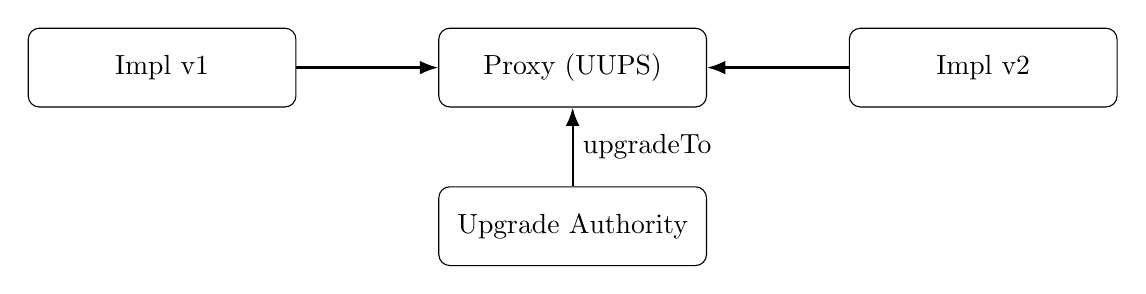
\begin{tikzpicture}[
  node distance=10mm,
  box/.style={draw, rounded corners, align=center, minimum width=34mm, minimum height=10mm},
  arr/.style={-Latex, thick}
]
\node[box] (impl1) {Impl v1};
\node[box, right=18mm of impl1] (proxy) {Proxy (UUPS)};
\node[box, below=10mm of proxy] (admin) {Upgrade Authority};
\node[box, right=18mm of proxy] (impl2) {Impl v2};

\draw[arr] (impl1) -- (proxy);
\draw[arr] (admin) -- node[right]{upgradeTo} (proxy);
\draw[arr] (impl2) -- (proxy);
\end{tikzpicture}
\caption{UUPS upgrade flow (vue simplifiée)}
\label{fig:uups_flow}
\end{figure}

\subsection*{Figure --- From code to mainnet (verification \& monitoring)}
\begin{figure}[h]
\centering
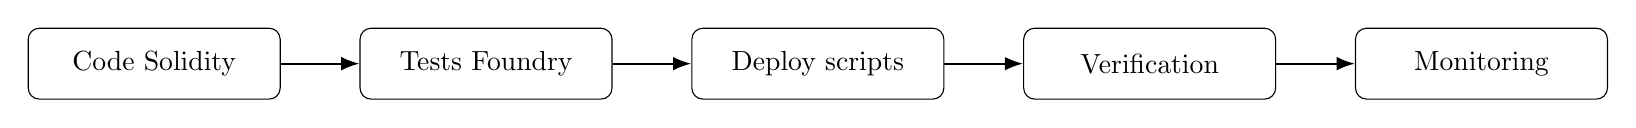
\begin{tikzpicture}[
  node distance=8mm,
  box/.style={draw, rounded corners, align=center, minimum width=32mm, minimum height=9mm},
  arr/.style={-Latex, thick}
]
\node[box] (code) {Code Solidity};
\node[box, right=10mm of code] (tests) {Tests Foundry};
\node[box, right=10mm of tests] (deploy) {Deploy scripts};
\node[box, right=10mm of deploy] (verify) {Verification};
\node[box, right=10mm of verify] (monitor) {Monitoring};

\draw[arr] (code) -- (tests);
\draw[arr] (tests) -- (deploy);
\draw[arr] (deploy) -- (verify);
\draw[arr] (verify) -- (monitor);
\end{tikzpicture}
\caption{Chaîne industrielle : code $\rightarrow$ tests $\rightarrow$ deploy $\rightarrow$ verify $\rightarrow$ monitoring}
\label{fig:code_to_mainnet}
\end{figure}

\end{document}
